%% LyX 2.3.4.2 created this file.  For more info, see http://www.lyx.org/.
%% Do not edit unless you really know what you are doing.
\documentclass[UTF8]{ctexart}
\usepackage[T1]{fontenc}
\usepackage{geometry}
\usepackage{graphicx}
\geometry{verbose,tmargin=3cm,bmargin=3cm,lmargin=2cm,rmargin=2cm,headheight=1cm,headsep=1cm}
\usepackage{float}
\usepackage{amstext}
%\setlength{\parindent}{0pt}
\usepackage{hyperref}
\usepackage{listings}
\usepackage{xcolor}

\makeatletter
\providecommand{\tabularnewline}{\\}
\DeclareRobustCommand\nobreakspace{\leavevmode\nobreak\ }

\makeatother

\begin{document}
\title{典型单纯李群的表示}
\date{任杰}

\maketitle
\noindent 单纯李代数可分为 4 类典型李代数和 5 个例外李代数。其中 4 类典型李代数为:
\begin{itemize}
	\item 特殊幺正群 SU(n) 对应的$A_{n-1}$代数;
	\item 特殊正交群 SO(2n+1) 对应$B_n$代数;
	\item 特殊正交群 SO(2n) 对应$D_n$代数;
	\item 幺正辛群 USp(2n) 对应的$B_n$代数。
\end{itemize}
本文讨论这 4 类典型单纯李代数的线性不可约表示。本文对李代数不可约表示的一般构造方法不多做介绍,这部分内容不同教科书中已有十分详细的介绍。我本人喜欢用具体的例子来直观理解较为抽象的概念,这也是本文的初衷。我把一些繁琐的公式和机械的计算总结成了一个 Mathematica package (\href{https://github.com/jayren3996/LieAlgebra}{jayren3996/LieAlgebra}),我们将借助它完成若干李群具体表示的计算。

作为凝聚态的学生,本人不十分关心李群在粒子物理或规范场论中的作用。对量子力学体系而言,对称群最主要的作用是将希尔伯特空间“分割”成彼此不正交的“块”。对于凝聚态体系,这个对称群可以是离散的点群、空间群,也可以是连续的 SO(3) 旋转群甚至秩更高的李群。我们也可以反过来,设计哈密顿量使得其具有某个李群对称性,或是包含若干个不可约表示空间作为不变子空间 (小广告: \href{https://arxiv.org/abs/2007.10380}{arxiv.2007.10380})。

李代数表示一般有两种平行的办法,一种是通过分析代数的根系,通过从最高权态出发在权上减去素根扩展得到新的权态,不同权态及它们的连接构成了权图。这种较为抽象的处理方法对较小的问题可以快速得到表示,但每个权态的意义不明确,尤其在出现重权情况较难分析;另一种方法是利用李群的张量表示,通过张量杨表得到不可约表示。这种方法相比之下操作手续更多,但每个态有明确的“物理意义”,重权分析也比较清晰。

本文主要讨论后一种办法,并重点强调张量表示和张量杨表的“物理意义”——张量表示就是群在多体希尔伯特空间上的表示,而张量杨表就是一个多体波函数。以下内容,我们会对 4 类典型李代数做具体讨论。首先将具体李代数基础表示看作一个有限能级的量子力学系统,再考虑生成元在多体波函数上的作用。

\section*{张量杨表与多体波函数}
\noindent 张量表示的定义是对于一个给定张量$T_{a_1,a_2,\cdots,a_N}$, 在群作用下“像张量那样变换”:
\begin{equation}
	(O_uT){a_1,\cdots,a_n} = \sum{b_1,\cdots b_N} u_{a_1,b_1}\cdots u_{a_N,b_N} T_{b_1,\cdots,b_N}, 
\end{equation}
其中每个$u_{a_i,b_i}$是群的一个基础表示。等价的表述是群作用可以分解为一系列基础表示的直积:
\begin{equation}
	O_u(g) = u_1(g)\otimes u_2(g) \otimes \cdots \otimes u_N(g).
\end{equation}
这正是多体系统中 onsite 对称性的形式。我们知道,N 体系统的多体波函数可以看作一个 N 阶张量,多体希尔伯特空间本身是每个格点上小希尔伯特空间的直积。这样我们建立了张量表示和多体希尔伯特空间表示的对应。

对于作用在 N 格点上的 onsite 对称性,简并波函数就自然构成了群的一个$d^N$表示,这个表示一般是可约的。而借助杨图方法我们可以具体得到张量空间中各个不可约表示。同理,杨图方法得到的不可约表示基底就对应希尔伯特空间中的一组波函数基底。

那么如何得到波函数呢?在张量表示中,不可约表示空间的态是用张量杨表给出的。每个张量杨表由一个正则杨算符作用在一个张量基底上得到,作用后得到另一个对称化的张量,这个张量就是多体波函数。举例而言,张量杨表

\begin{figure}[H]
\begin{centering}
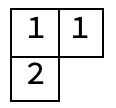
\includegraphics[width=.1\linewidth]{include/Y1}
\par\end{centering}
\end{figure}

\noindent 可以看作正则杨算符

\begin{figure}[H]
\begin{centering}
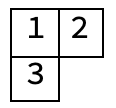
\includegraphics[width=.1\linewidth]{include/Y2}
\par\end{centering}
\end{figure}

\noindent 作用在张量基$\Psi_{1,1,2}$上得到,杨算符是一个置换操作,作用的结果为:
\begin{equation}
	2 \Psi_{1,1,2} - \Psi_{1,2,1} - \Psi_{2,1,1}. 
\end{equation}
这是一个对称化的张量,也是一个 3 粒子波函数。同时,这个张量杨表也可以表示为另一个正则杨算符

\begin{figure}[H]
\begin{centering}
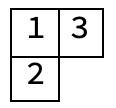
\includegraphics[width=.1\linewidth]{include/Y3}
\par\end{centering}
\end{figure}

\noindent 作用在另一个张量基$\Psi_{1,2,1}$上得到的张量:
\begin{equation}
	-\Psi_{1, 1, 2} + 2 \Psi_{1, 2, 1} - \Psi_{2, 1, 1}. 
\end{equation}
这两个波函数不相同,也不正交。但可以证明,不同正则杨算符对应出的张量(波函数)是线性无关的。以下我们约定,张量杨表默认对应最小杨算符(按顺序填充杨图)作用生成的波函数。

\section*{SU(N) 群李代数的表示}
\noindent 现在我们开始具体的例子。我们讨论主要讨论 SU(3) 群,更高的 SU(N) 群相比没有本质区别。在此我们简单介绍 Mathematica package 的用法。将文件ClassicalLieAlgebra.wl 放在某个文件夹中,在同一个文件夹新建一个 .nb 笔记本文件,在第一行输入运行导入命令:
\begin{verbatim}
	Import[NotebookDirectory[]<>"ClassicalLieAlgebra.wl"];
\end{verbatim}
这个 package 第一个功能是告诉我们代数生成元的具体信息,比如得到 SU(3) 标准生成元的命令为:
\begin{verbatim}
	MatrixForm /@ Generators[SU[3]]
\end{verbatim}
结果得到 8 个 Gell-Mann 矩阵:

\begin{figure}[H]
\begin{centering}
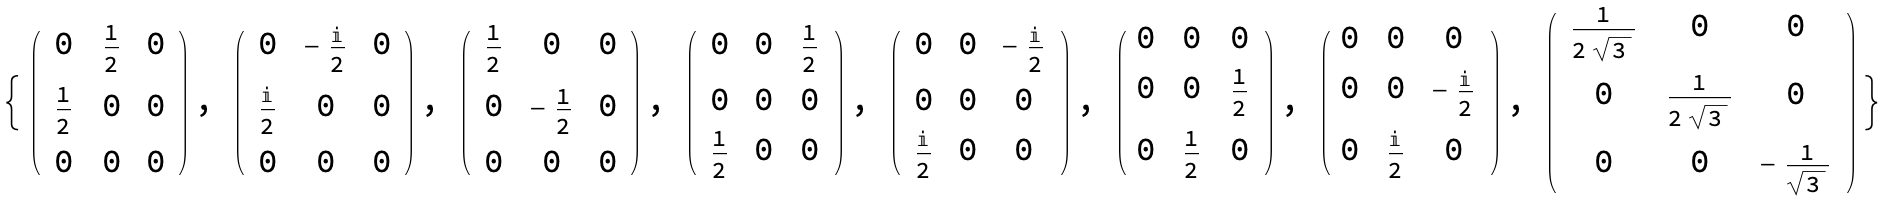
\includegraphics[width=0.95\linewidth]{include/O1}
\par\end{centering}
\end{figure}

\noindent 我们还可以用如下命令得到此代数的 Cartan-Weyl 基:
\begin{verbatim}
	{h, e, f} = CartanWeyl[SU[3]];
	Print["H = ", MatrixForm /@ h, ", E = ", MatrixForm /@ e, ", F = ", MatrixForm /@ f];
\end{verbatim}

\begin{figure}[H]
%\begin{centering}
\noindent 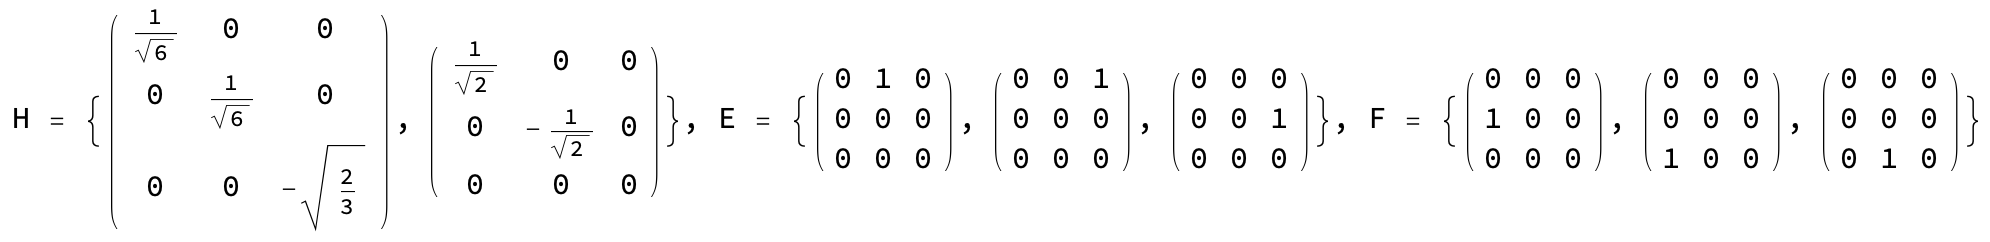
\includegraphics[width=0.95\linewidth]{include/O2}
%\par\end{centering}
\end{figure}

\noindent 对建立表示而言,最有用的生成元基底是 Chevalley,其具体形式为:

\begin{verbatim}
	{h, e, f} = Chevalley[SU[3]];
	Print["H = ", MatrixForm /@ h, ", E = ", MatrixForm /@ e, ", F = ", MatrixForm /@ f];
\end{verbatim}

\begin{figure}[H]
\begin{centering}
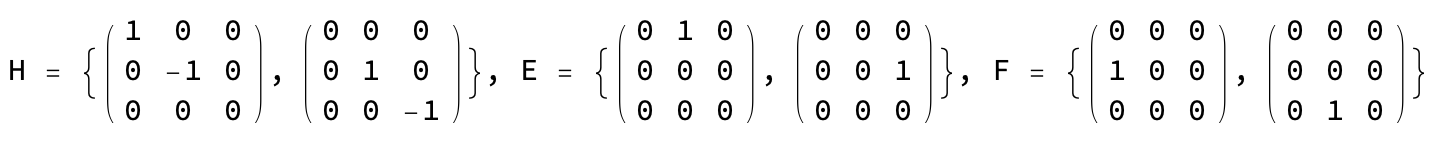
\includegraphics[width=0.95\linewidth]{include/O3}
\par\end{centering}
\end{figure}

\noindent 我们看到,Chevalley 基下生成元构成了两个耦合在一起的 SU(2),它们的关系可以直观表达为一个 3 能级系统的跃迁:

\begin{figure}[H]
\begin{centering}
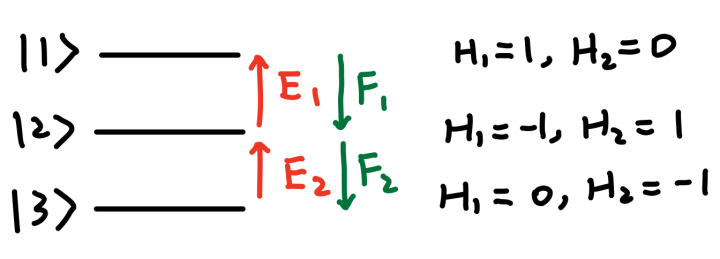
\includegraphics[width=0.5\linewidth]{include/P1}
\par\end{centering}
\end{figure}

\noindent 我们看到,3 类 Chevalley 基生成元在此 3 能级体系作用效果为:
\begin{itemize}
	\item $E_1,E_2$是能级上升算符,$F_1,F_2$是能级下降算符;
	\item $E_1,F_1,H_1$构成$\left| 1 \right \rangle, \left| 2 \right \rangle$之间的 SU(2) 代数,$E_2,F_2,H_2$构成$\left| 2 \right \rangle, \left| 3 \right \rangle$之间的 SU(2) 代数。
	\item $H_1,H_2$相当于这个 3 能级系统的两个“磁量子数”,各个能级有$H_1, H_2$确定的本征值;
	\item 从$H_1,H_2$的本征值看,$E_1$增加磁量子数为$(2,-1)$,而$E_2$增加磁量子数为$(-1,2)$.相应的,$F_1,F_2$算符减少对应的磁量子数。
\end{itemize}
这个 3 能级系统给出了 SU(3) 的基础表示。要得到更大的表示,我们只需要考虑 N 个这样的 3 能级系统在生成元作用下给出的表示。对于 N 体系统,总生成元为:
\begin{equation}
	H = \sum_i H_i ,  E = \sum_i E_i ,  F = \sum_i F_i. 
\end{equation}
总磁量子数可以用来标记表示中不同的态。这也被称为态的权(weight),权值不同的态一定是正交的。但有时表示空间中某些权值会有几个线性独立的态,这些态之间可能不正交,这时我们就遇到了重权问题。此时需要对权空间进行正交化。正交化的手续和量子力学中类似。
\subsection*{最高权张量杨表与波函数}
\noindent 要得到一个不可约表示空间,我们实际上只需要从这个空间的任意一个波函数出发,不断作用群生成元,生成的封闭空间就是不可约表示空间。因此 SU(3) 不可约表示最重要的是找到每个不可约表示空间的一个态。

而张量杨表就给出了这样一个态,即不可约表示的最高权态。SU(3) 群不可约表示可用不超过两行的杨表 $[\lambda_1, \lambda_2]$ 表示,对应的表示标记为 $(\lambda_1-\lambda_2,\lambda_3)$. 表示的指标代表最高权态的权值,或最高权态的“磁量子数”(由 Chevalley 基生成元 $H_i$ 本征值确定)。每个表示最高权态的张量杨表是在这个杨图第 1 行全部填 1,第二行全部填 2. 比如,对$(1,1)$表示,其张量杨表为:

\begin{figure}[H]
\begin{centering}
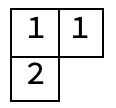
\includegraphics[width=0.1\linewidth]{include/Y1}
\par\end{centering}
\end{figure}

\noindent 这个张量杨表对应波函数可以用以下命令实现:
\begin{verbatim}
	ct = Tableau[{{1, 2}, {3}}];
v = Psi[1, 1, 2];
TableauPermute[ct, v]
\end{verbatim}
输出结果为
\begin{verbatim}
	2 Psi[1,1,2] - Psi[1,2,1] - Psi[2,1,1]
\end{verbatim}
也就是说,对于 SU(3) 的 $(l_1,l_2)$ 表示,形状为 $[l_1+l_2,l_2]$ ,并按上述规则填充的张量杨表就是这个表示的最高权态。

接下来,我们只要不断地将生成元作用在最高权态上,直至不能得到更多线性无关的波函数为止,就能得到表示空间。从这里开始,我们事实上可以完全在波函数上完成接下来的计算。但我们还是保留张量杨表的形式,因为它提供了多体波函数一个“紧凑”的形式,同时,张量杨表直观展示了波函数的一些置换对称性。比如由于杨算符列元素全反对称,张量杨表同一列不能填两个相同数字,否则波函数为 0.

\subsection*{生成 SU(3) 的 (1, 1) 表示空间}
\noindent 现在,我们从最高权态开始,作用 Chevalley 基下的两个生成元到这个波函数上,作用得到新的波函数相当于在生成元作用下的一次“跃迁”过程,我们可以用连线代表一个“跃迁”过程(单线代表 $F_1$ 作用,双线代表 $F_2$ 作用)。我们在此暂时不讨论跃迁矩阵元大小,第一级“跃迁”结果为:

\begin{figure}[H]
\begin{centering}
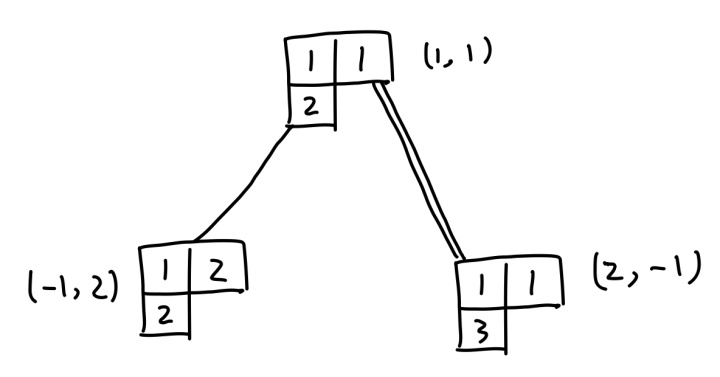
\includegraphics[width=0.5\linewidth]{include/T1}
\par\end{centering}
\end{figure}

\noindent 其中我们在每个张量杨表旁边标注了每个态的权(权值计算可以通过把每个小格子的磁量子数加起来,也可以通过从最高权计算降算符对权改变量得到)。

现在我们开始考虑第 2 级,注意左边的态

\begin{figure}[H]
\begin{centering}
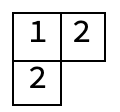
\includegraphics[width=0.1\linewidth]{include/Y4}
\par\end{centering}
\end{figure}

\noindent 在 $F_1$ 作用下消灭(同列出现相同数字),在 $F_2$ 作用下变成两个张量杨表的叠加态:

\begin{figure}[H]
\begin{centering}
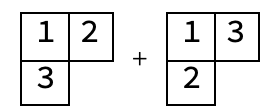
\includegraphics[width=0.25\linewidth]{include/Y5}
\par\end{centering}
\end{figure}

\noindent 而右边的态

\begin{figure}[H]
\begin{centering}
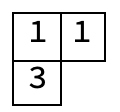
\includegraphics[width=0.1\linewidth]{include/Y6}
\par\end{centering}
\end{figure}

\noindent 在 $F_2$ 作用下消灭(张量杨表没有处现数字2),而由 $F_1$ 作用得到的态为:

\begin{figure}[H]
\begin{centering}
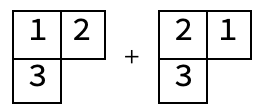
\includegraphics[width=0.25\linewidth]{include/Y7}
\par\end{centering}
\end{figure}

\noindent 第二张表不是正则杨表,右边的可以用杨算符对称性(1 分别和 2,3 交换)

\begin{figure}[H]
\begin{centering}
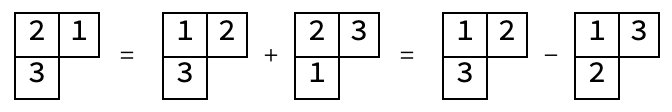
\includegraphics[width=0.6\linewidth]{include/Y8}
\par\end{centering}
\end{figure}

\noindent 化为正则张量杨表,最后为:

\begin{figure}[H]
\begin{centering}
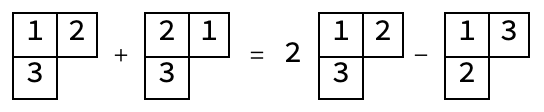
\includegraphics[width=0.5\linewidth]{include/Y9}
\par\end{centering}
\end{figure}

\noindent 此时,第 3 级得到的两个波函数

\begin{figure}[H]
\begin{centering}
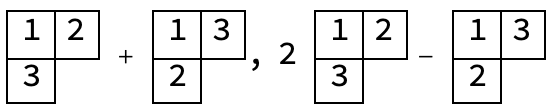
\includegraphics[width=0.5\linewidth]{include/Y10}
\par\end{centering}
\end{figure}

\noindent 的权均为 $(0,0)$ , 这提示遇到重权情况,这时我们需要权空间作正交化。和量子力学的正交化一样,基底的选取不唯一。习惯的选取是保留指标较小的生成元生成的态,将其他态相对这个态正交化。在这里对应保留右边的态。现在,我们可以把这两个杨表化为波函数做正交化。这个机械的手续可通过 Mathematica package 完成。首先建立两个张量杨表:
\begin{verbatim}
	a = 2 TensorTableau[{{1, 2}, {3}}] - TensorTableau[{{1, 3}, {2}}];
b = TensorTableau[{{1, 3}, {2}}] + TensorTableau[{{1, 2}, {3}}];
\end{verbatim}
正交化函数为:
\begin{verbatim}
	{c, d} = TableauOrthogonalization[a, b];
\end{verbatim}
最终我们可以打印出结果:
\begin{verbatim}
	TableauForm /@ {c, d}
\end{verbatim}

\begin{figure}[H]
\begin{centering}
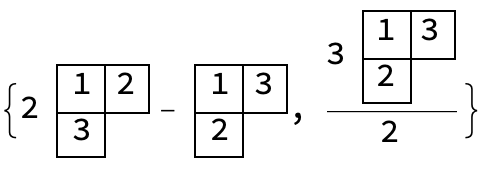
\includegraphics[width=0.4\linewidth]{include/O4}
\par\end{centering}
\end{figure}

\noindent 这样,我们将图画到了第 3 级:

\begin{figure}[H]
\begin{centering}
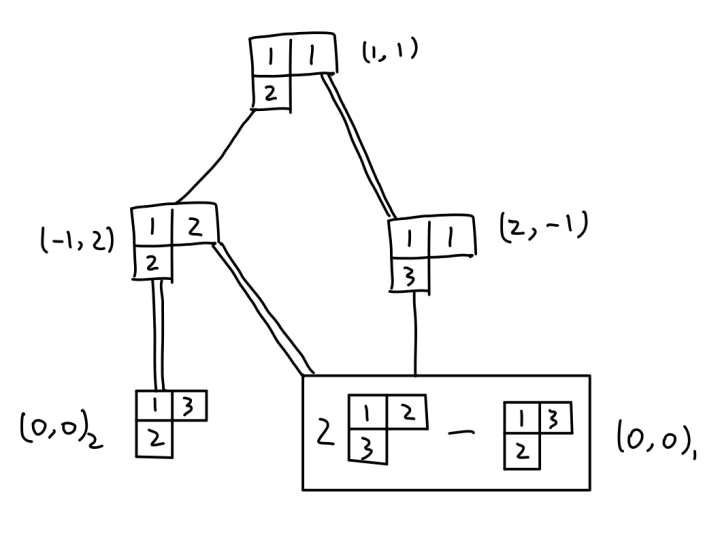
\includegraphics[width=0.5\linewidth]{include/T2}
\par\end{centering}
\end{figure}

\noindent 通常来说,这样的网络图在中间位置是最复杂的,接下去的两步就简单不少。由于没有出现重权,没有需要特别处理的地方,我们之间画出最后的图:

\begin{figure}[H]
\begin{centering}
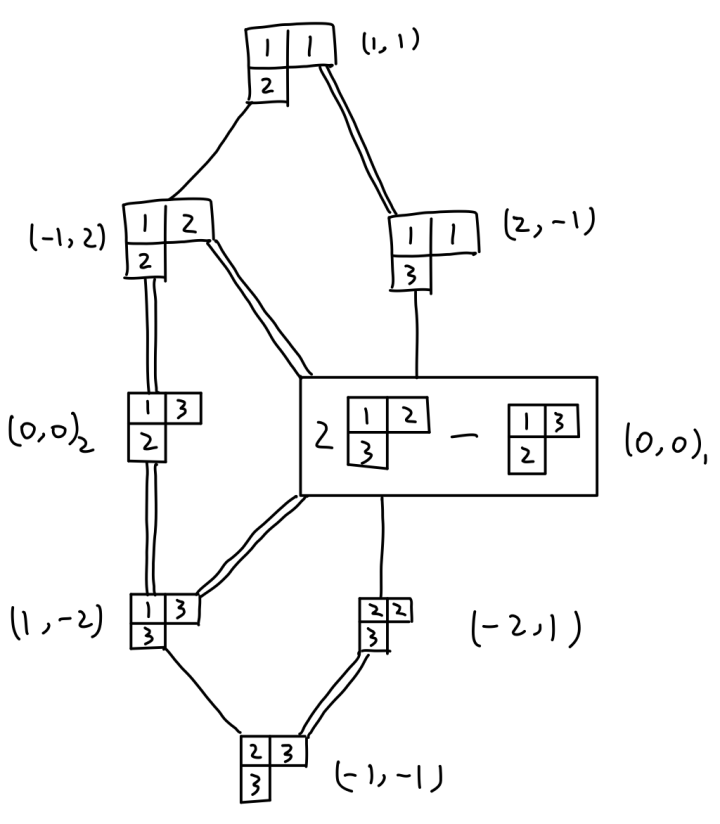
\includegraphics[width=0.5\linewidth]{include/T3}
\par\end{centering}
\end{figure}

\noindent 这样我们就得到 SU(3) 李代数 (1,1) 表示的结构图,我们看到这是一个 8 维空间,8 个节点给出了这个空间一组正交基底。同时两个生成元在此空间基底态之间可能产生的跃迁行为也由这张结构图确定。

现在还剩下一个问题,就是生成元在这些节点之间跃迁矩阵元的大小。这其实也类似一个量子力学问题。跃迁的系数很大程度是由每个态的归一化决定的。我们这里具体分析一个跃迁过程,即上图中:

\begin{figure}[H]
\begin{centering}
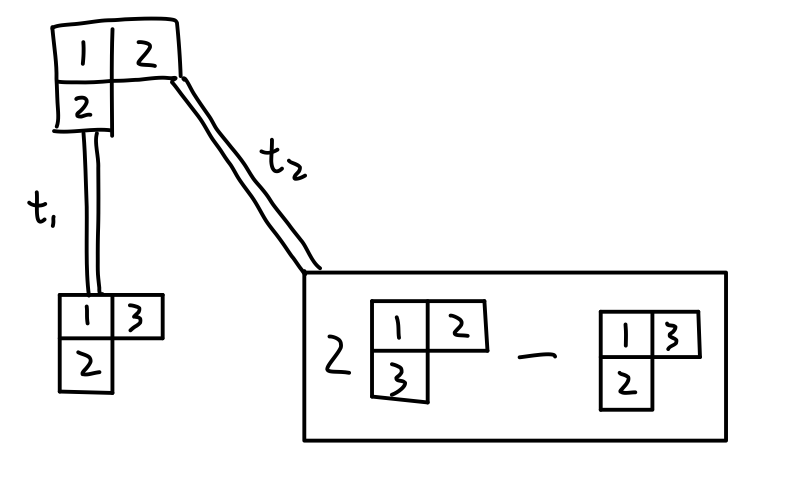
\includegraphics[width=0.4\linewidth]{include/T4}
\par\end{centering}
\end{figure}

\noindent 我们先从态

\begin{figure}[H]
\begin{centering}
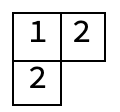
\includegraphics[width=0.1\linewidth]{include/Y4}
\par\end{centering}
\end{figure}

\noindent 出发,将这个态记为 $\left| a \right \rangle$,首先通过以下命令将其归一化:
\begin{verbatim}
	a = TensorTableau[{{1, 2}, {2}}];
na = TableauNormalization[a];
Print["|a> = ", TableauForm[na]];
\end{verbatim}

\begin{figure}[H]
\begin{centering}
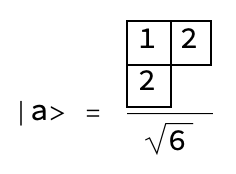
\includegraphics[width=0.25\linewidth]{include/O5}
\par\end{centering}
\end{figure}

\noindent 作用生成元 $F_2$ 的结果为:

\begin{figure}[H]
\begin{centering}
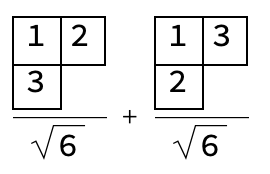
\includegraphics[width=0.25\linewidth]{include/O6}
\par\end{centering}
\end{figure}

\noindent 我们将这个态记为 $\left| b \right \rangle$ ,跃迁后两个基底态记为 $\left| c \right \rangle,\left| d \right \rangle$. 我们首先归一化 $\left| c \right \rangle,\left| d \right \rangle$ 态,再分别求内积,这部分计算可用以下命令实现(同时显示归一化的态):

\begin{verbatim}
	b = TensorTableau[{{1, 2}, {3}}]/Sqrt[6] + TensorTableau[{{1, 3}, {2}}]/Sqrt[6];
c = TensorTableau[{{1, 3}, {2}}];
d = 2 TensorTableau[{{1, 2}, {3}}] - TensorTableau[{{1, 3}, {2}}];
nc = TableauNormalization[c];
nd = TableauNormalization[d];
Print["|c> = ", TableauForm[nc], ", |d> = ", TableauForm[nd], ", |d> = ", TableauForm[nd],
 ", <d|b> = ", TableauDot[nd, b]];
\end{verbatim}

\begin{figure}[H]
\begin{centering}
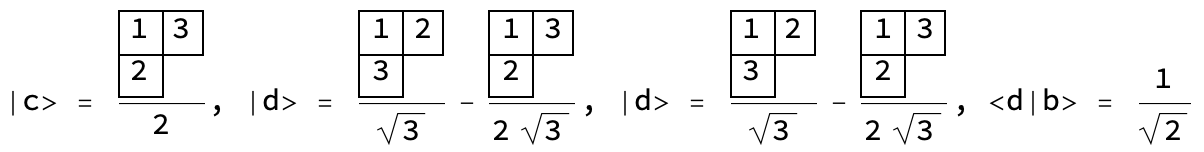
\includegraphics[width=0.95\linewidth]{include/O7}
\par\end{centering}
\end{figure}

\noindent 相应波函数内积就是跃迁矩阵元大小。

\subsection*{SU(4) 及更高秩代数}
\noindent 现在我们考虑更高的代数,首先我们观察几个更高秩的 SU(N) 在 Chevalley 基下的生成元:
\begin{verbatim}
	{h, e, f} = Chevalley[SU[4]];
Print["H = ", MatrixForm /@ h, ", E = ", MatrixForm /@ e, ", F = ", MatrixForm /@ f];
\end{verbatim}

\begin{figure}[H]
\begin{centering}
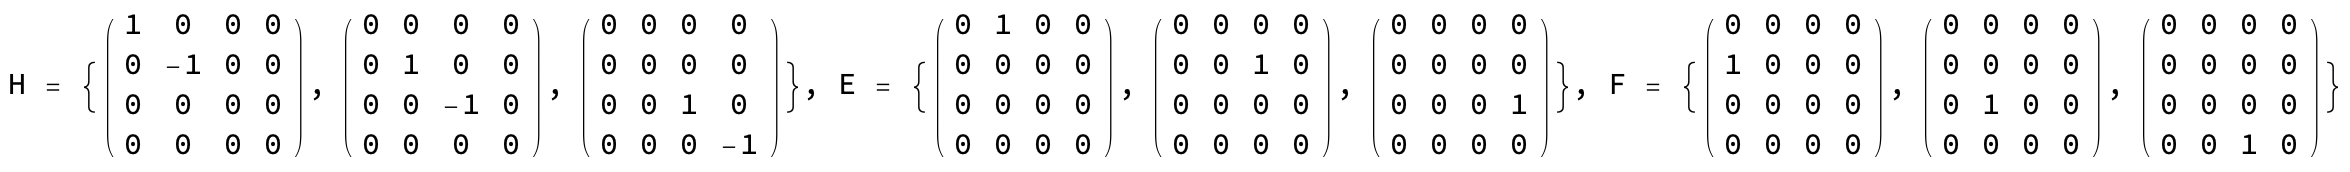
\includegraphics[width=0.95\linewidth]{include/O8}
\par\end{centering}
\end{figure}

\begin{verbatim}
	{h, e, f} = Chevalley[SU[5]];
Print["H = ", MatrixForm /@ h];
Print["E = ", MatrixForm /@ e];
Print["F = ", MatrixForm /@ f];
\end{verbatim}

\begin{figure}[H]
\begin{centering}
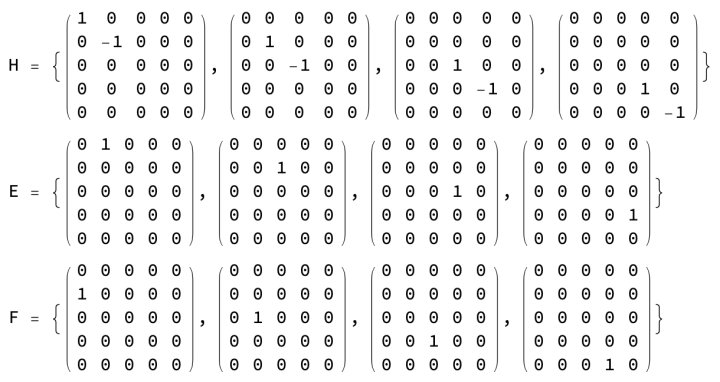
\includegraphics[width=0.6\linewidth]{include/O9}
\par\end{centering}
\end{figure}

\noindent 到这里,我们已经可以看出其中的规律,从 SU(3) 到 SU(4),变化仅是增加一个能级,加上相应的上升下降算符,并增加一个“磁量子数”算符,以此类推。

\begin{figure}[H]
\begin{centering}
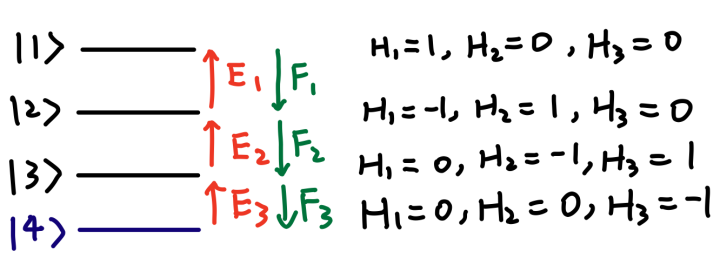
\includegraphics[width=0.5\linewidth]{include/P2}
\par\end{centering}
\end{figure}

\noindent 对 SU(4) 代数,我们举个最简单例子: $(0,1,0)$ 表示,最高权为:

\begin{figure}[H]
\begin{centering}
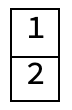
\includegraphics[width=0.06\linewidth]{include/Y11}
\par\end{centering}
\end{figure}

\noindent 构造过程不会出现重权情况,我们直接画出整张图:

\begin{figure}[H]
\begin{centering}
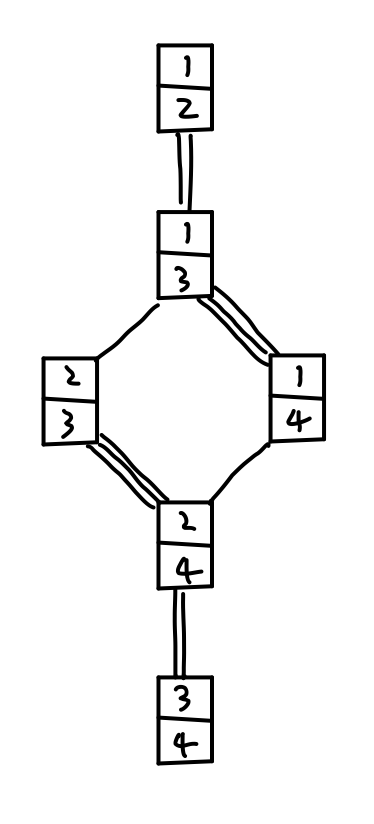
\includegraphics[width=0.3\linewidth]{include/T5}
\par\end{centering}
\end{figure}

\noindent 对 SU(N) 代数对讨论就到这里。下面我们分析其他三类典型李代数。构造表示空间的方法基本相同,至少生成元的具体形式发生了变化。

\section*{SO(2N+1) 群李代数的表示}
\noindent 现在我们来分析第 2 类典型李代数 SO(2N+1)。同样,我们首先看 SO(5) 生成元矩阵:
\begin{verbatim}
	MatrixForm /@ Generators[SO[5]]
\end{verbatim}

\begin{figure}[H]
\begin{centering}
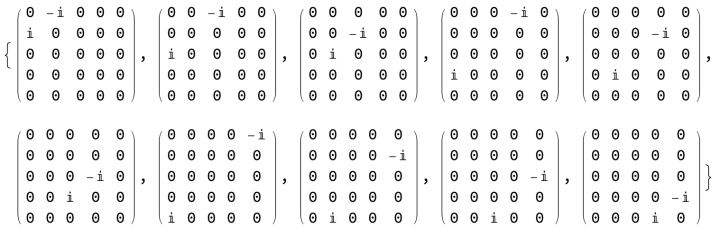
\includegraphics[width=0.8\linewidth]{include/O10}
\par\end{centering}
\end{figure}

\noindent 我们知道,SO(N) 标准生成元对应两个轴确定的“旋转”。但这组生成元不方便做李代数表示。我们通过以下命令

\begin{verbatim}
	{h, e, f} = Chevalley[SO[5]];
Print["H = ", MatrixForm /@ h];
Print["E = ", MatrixForm /@ e];
Print["F = ", MatrixForm /@ f];
\end{verbatim}
得到 Chevalley 基

\begin{figure}[H]
\begin{centering}
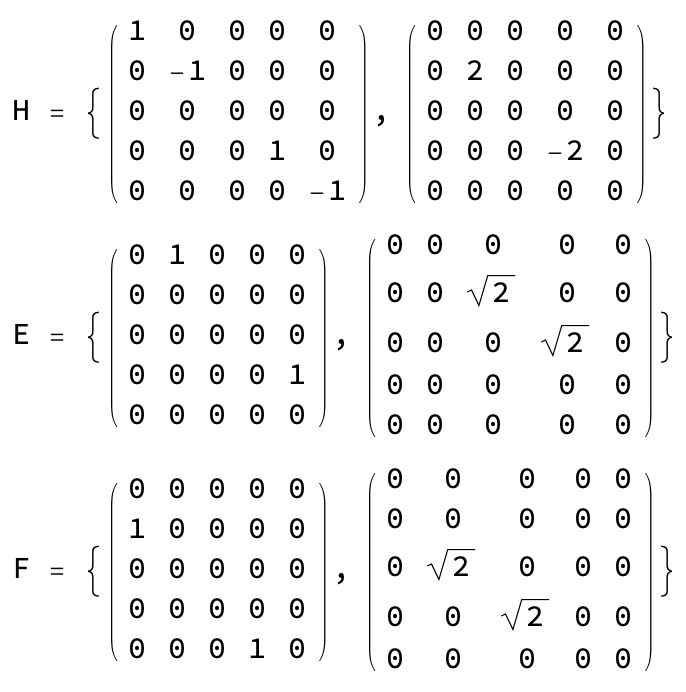
\includegraphics[width=0.4\linewidth]{include/O11}
\par\end{centering}
\end{figure}

\noindent 我们得到了想要的“能级跃迁”形式的生成元矩阵。注意 Chevalley 基的表示基底已从坐标基地变换为球谐基底,球谐基 5 个态具体形式为:

\begin{verbatim}
	MatrixForm/@StandardBasis[SO[5]]
\end{verbatim}

\begin{figure}[H]
\begin{centering}
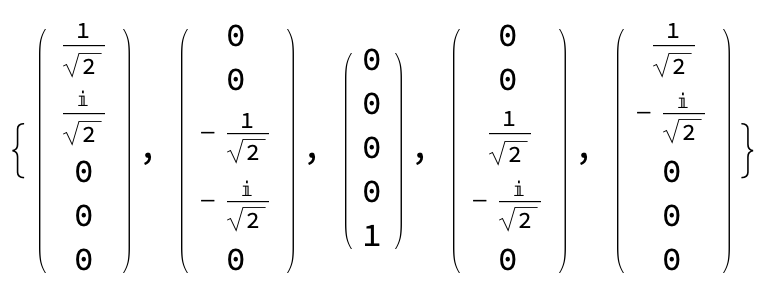
\includegraphics[width=0.4\linewidth]{include/O12}
\par\end{centering}
\end{figure}

\noindent 这样,SO(5) 基础表示可通过一个 5 能级系统表示出来:

\begin{figure}[H]
\begin{centering}
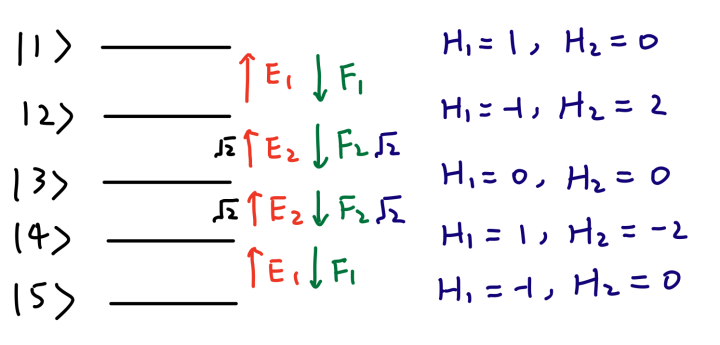
\includegraphics[width=0.5\linewidth]{include/P3}
\par\end{centering}
\end{figure}

\noindent 相比 SU(N),这里生成元的行为更复杂了些。如 $E_1,E_2$ 不再只作用于一个能级,而是能提升 $|2\rangle$ 或 $|5\rangle$ , $E_1,E_2$ 的系数也不再相同。同时“磁量子数”算符 $H_1,H_2$ 也不像 SU(N) 那样有规律,但除此之外,做法基本一样。

为了便于看出规律,我们再提高一级,观察 SO(7) 的生成元形式:
\begin{verbatim}
	{h, e, f} = Chevalley[SO[7]];
Print["H = ", MatrixForm /@ h];
Print["E = ", MatrixForm /@ e];
Print["F = ", MatrixForm /@ f];
\end{verbatim}

\begin{figure}[H]
\begin{centering}
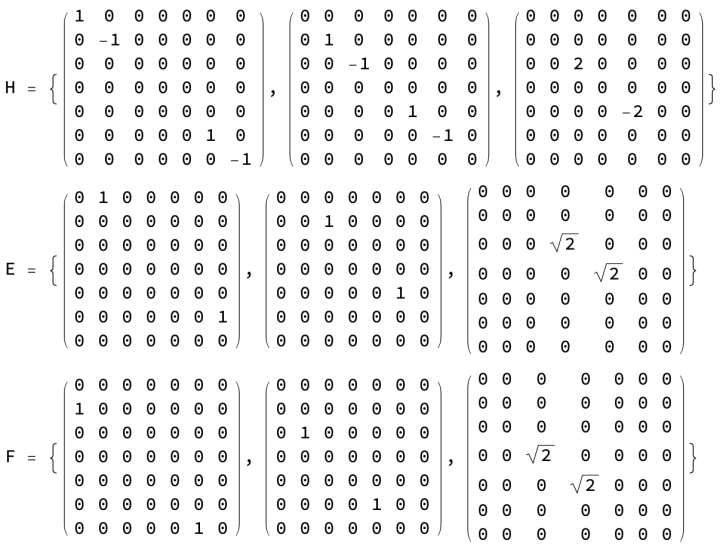
\includegraphics[width=0.8\linewidth]{include/O13}
\par\end{centering}
\end{figure}

\noindent 我们看到 $E_1,E_2$ 算符和 $E_3$ 算符的地位不同,生成元在这个 7 能级系统上作用效果为:

\begin{figure}[H]
\begin{centering}
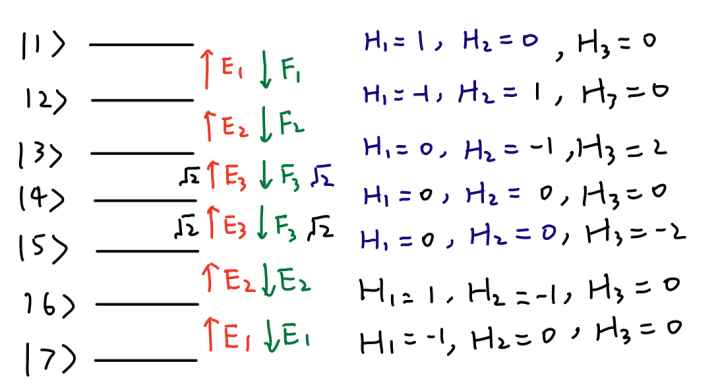
\includegraphics[width=0.7\linewidth]{include/P4}
\par\end{centering}
\end{figure}

\noindent 根据此规律,具体作一例如下。

\subsection*{生成 SO(7) 的 (2,0,0) 表示空间}

\noindent SO(2N+1) 的最高权态规律和 SU(N) 类似,只是我们考虑的是不超过 N 行的张量杨表(杨表最大行数由李代数的秩决定,即“磁量子数”算符 $H_i$ 的数量)。对形状为 $[\lambda_1 ,\cdots, \lambda_N]$ 的杨表,对应表示指标为 $(\lambda_1 - \lambda_2, \lambda_2-\lambda_3, \cdots,\lambda_{N-1}-\lambda_N, 2 \lambda_3)$,注意最后一个分量上的 2 倍。最高权张量杨表填充仍然是第 $i$ 行填数字 $i$. 我们现在考虑 SO(7) 上的 $(2,0,0)$ 表示,其最高权态为

\begin{figure}[H]
\begin{centering}
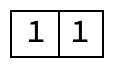
\includegraphics[width=0.15\linewidth]{include/Y12}
\par\end{centering}
\end{figure}

\noindent 从这个态开始,按规则作用生成元,我们无阻力地画到第 6 级:

\begin{figure}[H]
\begin{centering}
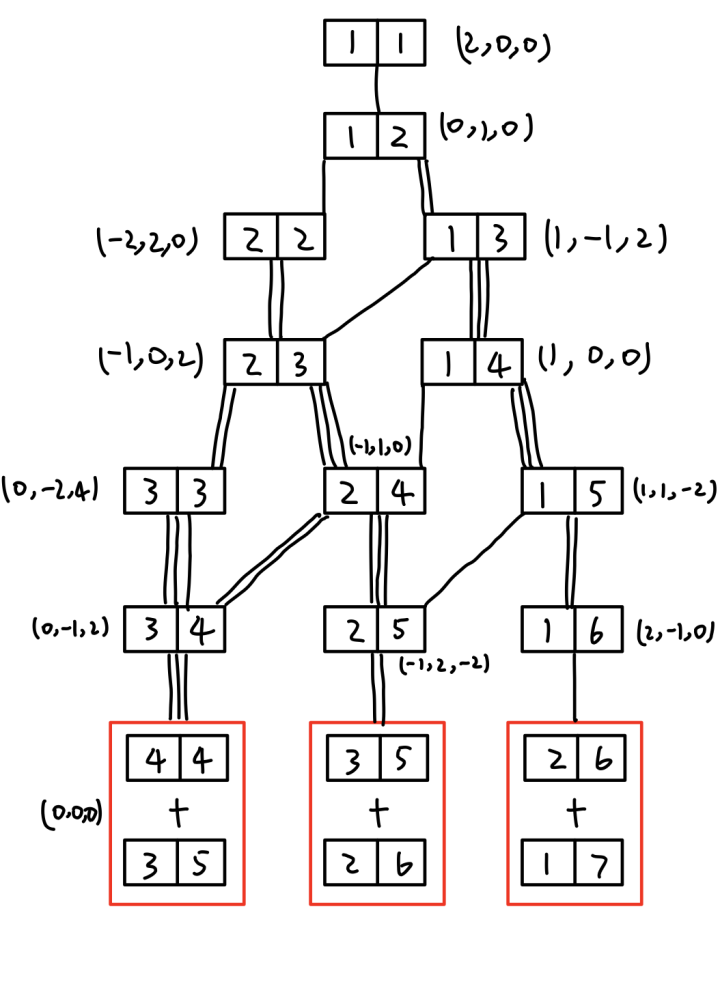
\includegraphics[width=0.5\linewidth]{include/T6}
\par\end{centering}
\end{figure}

\noindent 到第 7 级时,红框出现重权。开始正交化程序:

\begin{verbatim}
	a = TensorTableau[{{2, 6}}] + TensorTableau[{{1, 7}}];
b = TensorTableau[{{3, 5}}] + TensorTableau[{{2, 6}}];
c = TensorTableau[{{4, 4}}] + TensorTableau[{{3, 5}}];
{a, b} = TableauOrthogonalization[a, b];
{a, c} = TableauOrthogonalization[a, c];
{b, c} = TableauOrthogonalization[b, c];
TableauForm /@ {a, b, c}
\end{verbatim}

\begin{figure}[H]
\begin{centering}
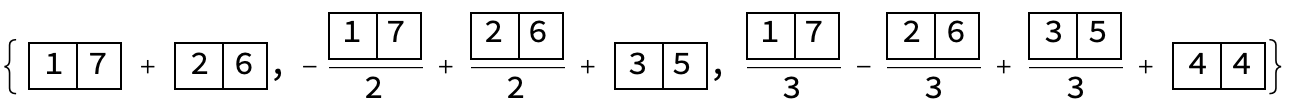
\includegraphics[width=0.95\linewidth]{include/O14}
\par\end{centering}
\end{figure}

\noindent 为了简化图,我们用 A,B,C 代表这三个正交的态。后面的图和前面是对称的,不会出现重权,我们补全剩余的图:

\begin{figure}[H]
\begin{centering}
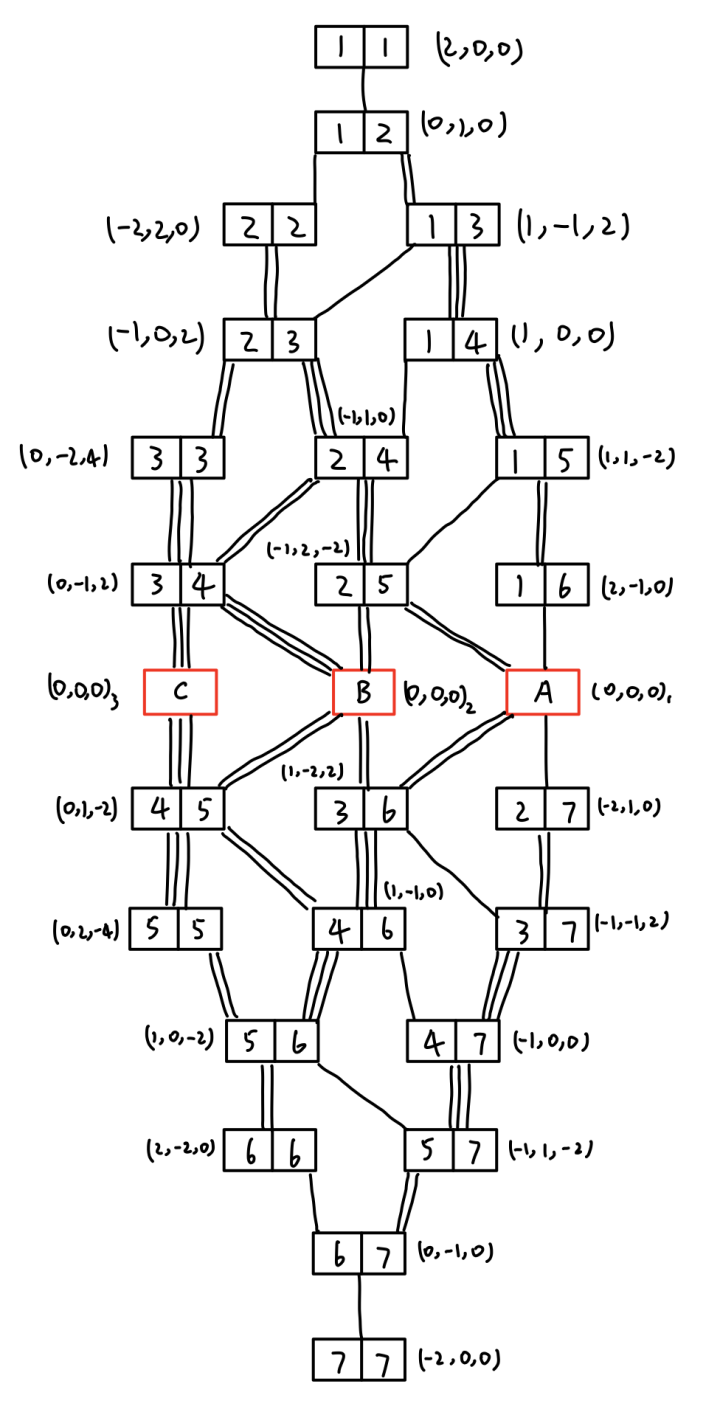
\includegraphics[width=0.5\linewidth]{include/T7}
\par\end{centering}
\end{figure}

\noindent 对 SO(2N+1) 代数表示讨论到这里。讨论 SO(N) 群李代数需要区分 N 的奇偶,我们接下来考虑偶数 N 的特殊正交群李代数。

\section*{SO(2N) 群李的表示}
\noindent 现在看第 3 类典型李代数 SO(2N),我们首先看 SO(4) 的 Chevalley 基生成元:
\begin{verbatim}
	{h, e, f} = Chevalley[SO[4]];
Print["H = ", MatrixForm /@ h, ", E = ", MatrixForm /@ e, ", F = ", MatrixForm /@ f];
\end{verbatim}
\begin{figure}[H]
\begin{centering}
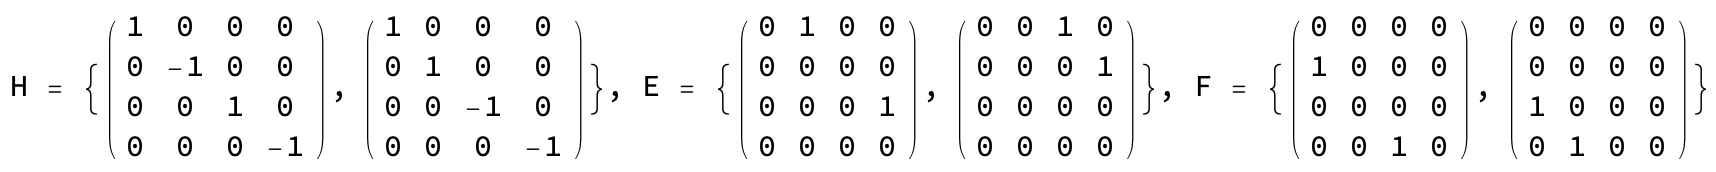
\includegraphics[width=0.95\linewidth]{include/O15}
\par\end{centering}
\end{figure}

\noindent 注意 Chevalley 基矩阵形式也是写在球谐基下的,相应基向量为:

\begin{verbatim}
	MatrixForm /@ StandardBasis[SO[4]]
\end{verbatim}

\begin{figure}[H]
\begin{centering}
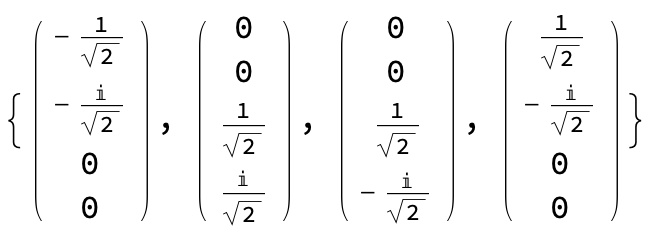
\includegraphics[width=0.5\linewidth]{include/O16}
\par\end{centering}
\end{figure}

\noindent 这组生成元作用对应一个 4 能级系统:

\begin{figure}[H]
\begin{centering}
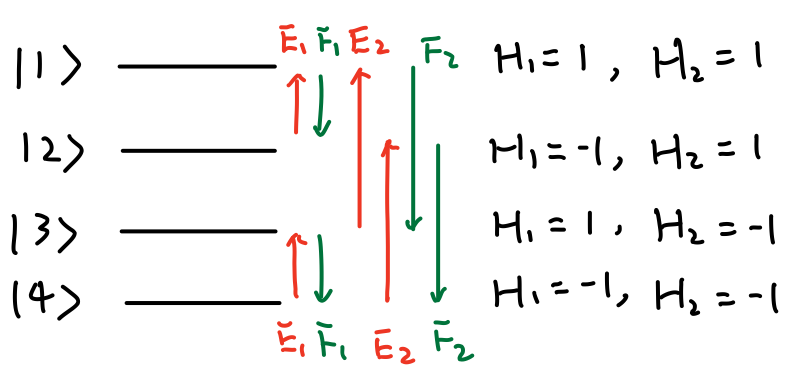
\includegraphics[width=0.5\linewidth]{include/P5}
\par\end{centering}
\end{figure}

\noindent 为进一步观察出规律,我们让程序打印出更 SO(6) 群生成元:

\begin{verbatim}
	{h, e, f} = Chevalley[SO[6]];
Print["H = ", MatrixForm /@ h];
Print["E = ", MatrixForm /@ e];
Print["F = ", MatrixForm /@ f];
\end{verbatim}

\begin{figure}[H]
\begin{centering}
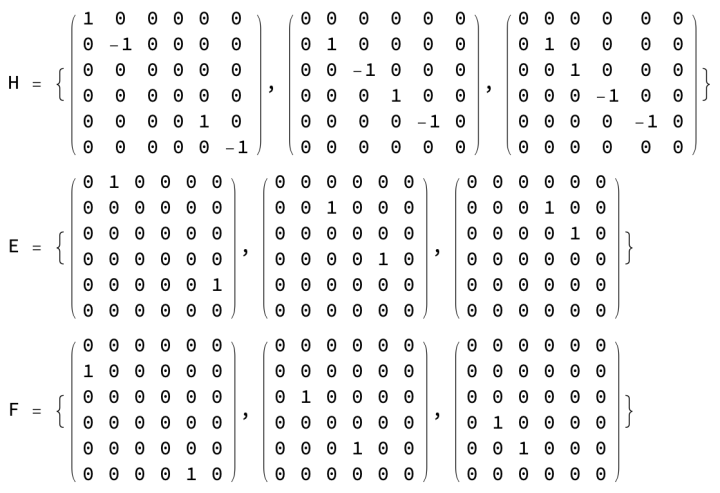
\includegraphics[width=0.7\linewidth]{include/O17}
\par\end{centering}
\end{figure}

\noindent 对应一个 6 能级系统

\begin{figure}[H]
\begin{centering}
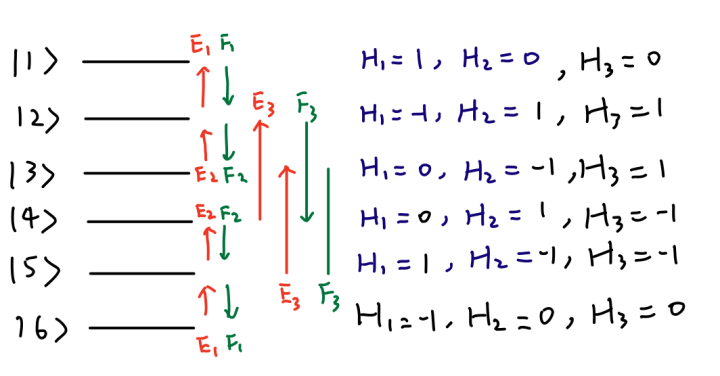
\includegraphics[width=0.6\linewidth]{include/P6}
\par\end{centering}
\end{figure}

\noindent SO(2N) 最高权的也类似地由不超过 N 行的杨图表示。当杨表行数小于 N,最高权张量杨表填充方式和 SU(N) 相同,即第  $i$  行全填数字  $i$ ,相应不可约表示指标为 $(\lambda_1 -\lambda_2, \cdots,\lambda_{N-2}-\lambda_{N-1},\lambda_{N-1}, \lambda_{N-1})$. 但是当杨表行数等于 N 时,第 N 行可以填入 N,也可以填入 N+1:填入 N 时,对应表示指标为 $(\lambda_1 - \lambda_2, \cdots, \lambda_{N-1} - \lambda_N,\lambda_{N-1} + \lambda_N )$;而填入 N+1 时,对应表示指标为 $(\lambda_{1} - \lambda_2, \cdots, \lambda_{N-1} + \lambda_N,\lambda_{N-1} - \lambda_N)$. 关于这点,我们也可以直接从最高权态“磁量子数”看出来。我们举相对小表示的例子。考虑 SO(6) 的 $(0,1,1)$ 表示,其最高权态为

\begin{figure}[H]
\begin{centering}
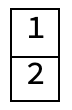
\includegraphics[width=0.06\linewidth]{include/Y11}
\par\end{centering}
\end{figure}

\noindent 我们将关系图推进到第 4 级:

\begin{figure}[H]
\begin{centering}
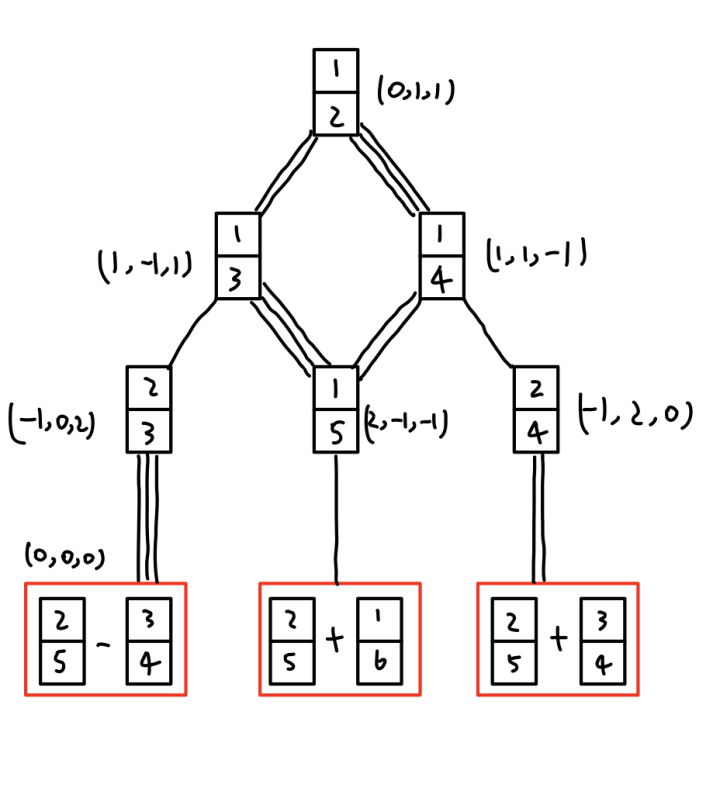
\includegraphics[width=0.6\linewidth]{include/T8}
\par\end{centering}
\end{figure}

\noindent 红框内出现了重权情况,进行正交化:

\begin{verbatim}
	a = TensorTableau[{{2}, {5}}] + TensorTableau[{{1}, {6}}];
b = TensorTableau[{{2}, {5}}] + TensorTableau[{{3}, {4}}];
c = TensorTableau[{{2}, {5}}] - TensorTableau[{{3}, {4}}];
{a, b} = TableauOrthogonalization[a, b];
{a, c} = TableauOrthogonalization[a, c];
{b, c} = TableauOrthogonalization[b, c];
TableauForm /@ {a, b, c}
\end{verbatim}

\begin{figure}[H]
\begin{centering}
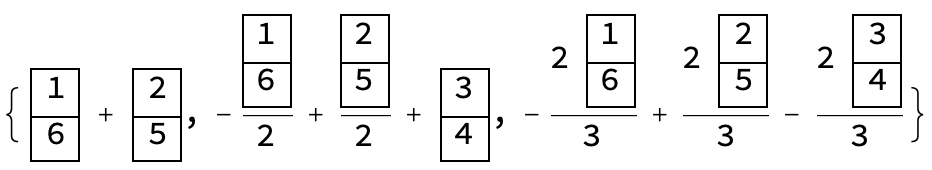
\includegraphics[width=0.8\linewidth]{include/O18}
\par\end{centering}
\end{figure}

\noindent 记为 A,B,C, 继续完成剩余半张图:

\begin{figure}[H]
\begin{centering}
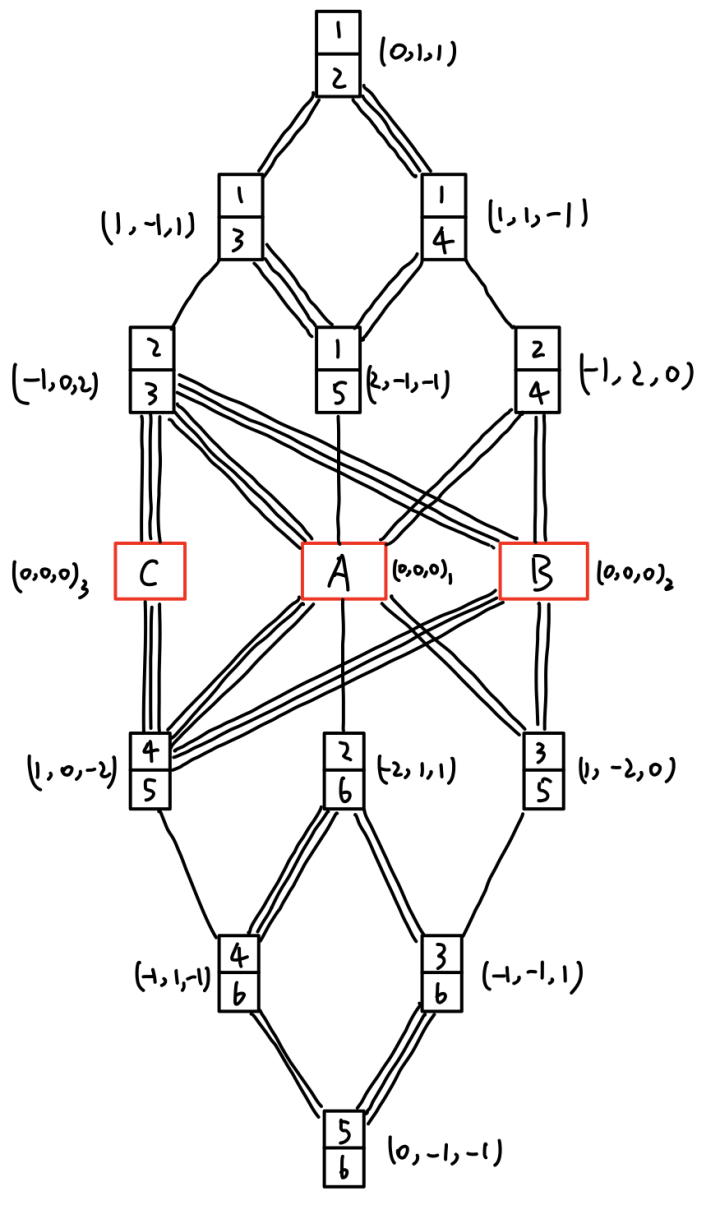
\includegraphics[width=0.6\linewidth]{include/T9}
\par\end{centering}
\end{figure}

\section*{USp(2N) 群李代数的表示}
\noindent 现在我们考虑最后一类典型李代数,USp(2N),即幺正的辛群的李代数。我们首先让程序打印出 USp(4) 的 Chevalley 基生成元:
\begin{verbatim}
	{h, e, f} = Chevalley[Sp[4]];
Print["H = ", MatrixForm /@ h, ", E = ", MatrixForm /@ e, ", F = ", MatrixForm /@ f];
\end{verbatim}

\begin{figure}[H]
\begin{centering}
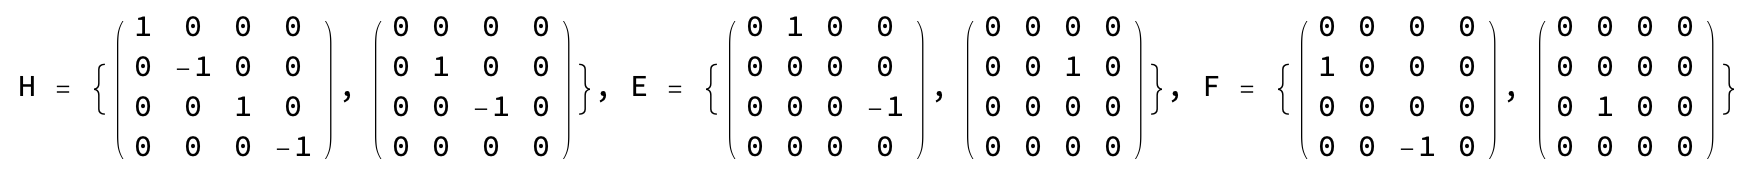
\includegraphics[width=0.95\linewidth]{include/O19}
\par\end{centering}
\end{figure}

\noindent 对应 4 能级系统:

\begin{figure}[H]
\begin{centering}
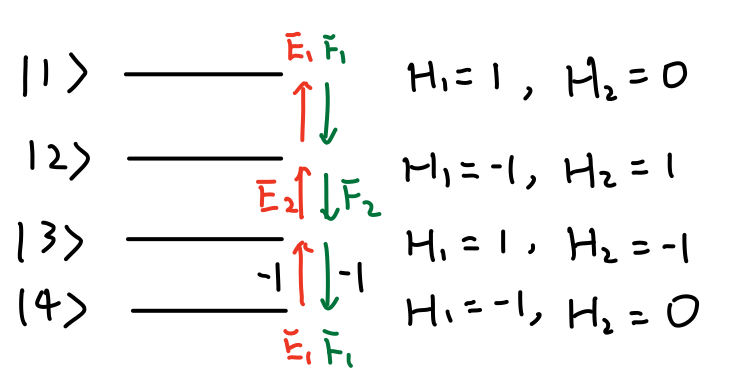
\includegraphics[width=0.5\linewidth]{include/P7}
\par\end{centering}
\end{figure}

\noindent 再看 USp(6) 生成元:

\begin{verbatim}
	{h, e, f} = Chevalley[Sp[6]];
Print["H = ", MatrixForm /@ h];
Print["E = ", MatrixForm /@ e];
Print["F = ", MatrixForm /@ f];
\end{verbatim}

\begin{figure}[H]
\begin{centering}
\includegraphics[width=0.6\linewidth]{include/O20}
\par\end{centering}
\end{figure}

\noindent 对应 6 能级系统:

\begin{figure}[H]
\begin{centering}
\includegraphics[width=0.5\linewidth]{include/P8}
\par\end{centering}
\end{figure}

\noindent USp(2N) 不可约表示的最高权态规则和 SU(N),SO(2N+1) 类似,至少杨图要求不超过 N 行。我们举 USp(6) 的 (0,1,0) 表示的例子。其最高权态为:

\begin{figure}[H]
\begin{centering}
\includegraphics[width=0.06\linewidth]{include/Y11}
\par\end{centering}
\end{figure}

\noindent 同样,我们无阻力地来到第 4 级:

\begin{figure}[H]
\begin{centering}
\includegraphics[width=0.5\linewidth]{include/T10}
\par\end{centering}
\end{figure}

\noindent 注意红框内叠加态符号是减,来源于上述“跃迁规则”出现的负号。同时,红框出现重权,要进行正交化手续:

\begin{verbatim}
	a = TensorTableau[{{2}, {5}}] - TensorTableau[{{1}, {6}}];
b = TensorTableau[{{3}, {4}}] - TensorTableau[{{2}, {5}}];
{a, b} = TableauOrthogonalization[a, b];
TableauForm /@ {a, b}
\end{verbatim}

\begin{figure}[H]
\begin{centering}
\includegraphics[width=0.5\linewidth]{include/O21}
\par\end{centering}
\end{figure}

\noindent 正交化后的态分别记为 A,B,再继续完成剩余半张图:

\begin{figure}[H]
\begin{centering}
\includegraphics[width=0.5\linewidth]{include/T11}
\par\end{centering}
\end{figure}

\section*{小结}
\noindent 通过对于 4 类典型李代数表示空间的具体计算,我们可以对典型李代数不可约表示空间构造有一个直观的认识。不同李代数的表示构造都由 4 个步骤完成:
\begin{itemize}
	\item 将张量杨表对应为波函数,利用相应的杨图填充规则就得到了某个不可约表示的最高权态。
	\item 不断对张量杨表作用下降算符,“跃迁”出新的态,同时记录它们的“磁量子数”,不同“磁量子数”的态一定是正交的。
	\item 有时,“跃迁”出的张量杨表不是正则的,就通过张量杨表的对称性将其化为正则张量杨表(的线性组合)。
	\item 当有多个态有相同的“磁量子数”,就要对相应“磁量子数”简并空间做正交化。

\end{itemize}
其中不同的李代数主要的区别在于生成元的“跃迁”规则。而这部分无需记忆,我们可以利用程序打印出 Chevalley 基下的生成元直接看出“跃迁规则”。

\subsection*{Reference}
\noindent [1] 马中骐. 物理学中的群论.

\noindent [2] H.Georgi. Lie algebras in particle physics.

\end{document}
